\documentclass[11pt,a4paper]{article}
\usepackage[utf8]{inputenc}
\usepackage[T1]{fontenc}
\IfFileExists{lmodern.sty}{\usepackage{lmodern}}{}
\IfFileExists{french.ldf}{\usepackage[french]{babel}}{\usepackage[english]{babel}}
\usepackage{amsmath,amssymb,amsfonts,amsthm}
\usepackage{geometry}
\geometry{top=2cm, bottom=2cm, left=2.2cm, right=2.2cm}
\usepackage{booktabs,array,multirow}
\usepackage{enumitem}
\usepackage{xcolor}
\usepackage{tcolorbox}
\tcbuselibrary{skins,breakable}
\usepackage{tikz}
\usetikzlibrary{arrows.meta,positioning,shapes.geometric,calc}
\usepackage[colorlinks=true,linkcolor=blue!60!black]{hyperref}
\newtcolorbox{propbox}[1]{colback=blue!5!white,colframe=blue!75!black,fonttitle=\bfseries,title={#1},breakable,boxrule=0.8pt}
\newtcolorbox{rembox}[1]{colback=orange!5!white,colframe=orange!80!black,fonttitle=\bfseries,title={#1},breakable,boxrule=0.8pt}
\newtcolorbox{verifbox}{colback=green!4!white,colframe=green!45!black,fonttitle=\bfseries,title=Vérification algorithmique (Python),breakable,boxrule=0.6pt}
\newcommand{\Xt}{\tilde{X}}
\newcommand{\Yt}{\tilde{Y}}
\setlength{\parindent}{0pt}
\setlength{\parskip}{4pt}
\usepackage{fancyhdr}
\pagestyle{fancy}\fancyhf{}
\lhead{\small Guide complet -- Théorie des Jeux}\rhead{\small Master RO -- Bouira 2025/2026}\cfoot{\thepage}
\setlength{\headheight}{14pt}
\newtcolorbox{methbox}[1]{colback=violet!4!white,colframe=violet!70!black,fonttitle=\bfseries,title={#1},breakable,boxrule=0.8pt}
\newtcolorbox{piegebox}{colback=red!4!white,colframe=red!70!black,fonttitle=\bfseries,title={Pièges classiques},breakable,boxrule=0.8pt}
\newtcolorbox{whenbox}{colback=yellow!8!white,colframe=yellow!50!black,fonttitle=\bfseries,title={Quand l'utiliser ?},breakable,boxrule=0.6pt}
\tikzset{
 q/.style={draw,rounded corners,fill=blue!8,align=center,font=\small,text width=#1},
 q/.default=3.6cm,
 m/.style={draw,fill=green!10,align=center,font=\small,text width=#1},
 m/.default=3.4cm,
 arr/.style={-{Stealth[length=2.2mm]},thick},
 lab/.style={font=\scriptsize,fill=white,inner sep=1pt}
}

\title{\textbf{Université Akli Mohand Oulhadj -- Bouira}\\
\large Master Recherche Opérationnelle -- 2025/2026\\[3mm]
\Huge \textbf{Guide Complet de Révision}\\[2mm]
\Large \textbf{Théorie des Jeux}\\[2mm]
\normalsize Cours (Chapitres 1 et 2) $\cdot$ Méthodes $\cdot$ Arbres de décision $\cdot$ Formulaire $\cdot$ QCM $\cdot$ Exercices résolus}
\author{Construit à partir des deux chapitres du cours, du corrigé officiel du DM1,\\ de la solution notée 20/20 et des corrigés TD1, TD2, DM2, Examen, Test.\\ Tous les résultats chiffrés sont vérifiés par \texttt{verification\_TDJ.py} (71 tests).}
\date{}

\begin{document}
\maketitle
\thispagestyle{empty}
\tableofcontents
\newpage

%=====================================================================
\section{Comment utiliser ce guide}
\begin{itemize}
\item \textbf{Veille d'examen} : la section~\ref{sec:arbres} (arbres de décision), la section~\ref{sec:formulaire} (formulaire) et la section~\ref{sec:pieges} (pièges).
\item \textbf{Exercice bloquant} : identifier le type de jeu avec l'arbre principal, puis appliquer la fiche méthode correspondante (sections~\ref{sec:methodes} et~\ref{sec:nash}).
\item \textbf{QCM} : section~\ref{sec:qcm} (faits à mémoriser et corrigé du Test).
\item \textbf{Entraînement} : section~\ref{sec:recap} (tous les exercices avec méthode et résultat) et section~\ref{sec:entrainement}.
\end{itemize}

\begin{rembox}{La rédaction qui rapporte tous les points (modèle du corrigé officiel et de la copie 20/20)}
Pour chaque question : \textbf{(1)} rappel du résultat de cours utilisé (définition ou théorème, avec page), \textbf{(2)} calcul détaillé et lisible, \textbf{(3)} conclusion \textbf{encadrée}, \textbf{(4)} vérification (Théorème 2 pour un jeu matriciel ; « aucune déviation profitable » pour Nash). Dire explicitement « large » ou « stricte » pour toute domination. Ne jamais oublier le gain du joueur 2 ($-v$) quand il est demandé.
\end{rembox}

%=====================================================================
\section{Arbres de décision}\label{sec:arbres}

\subsection{Arbre principal : quel type de jeu ?}
\begin{center}
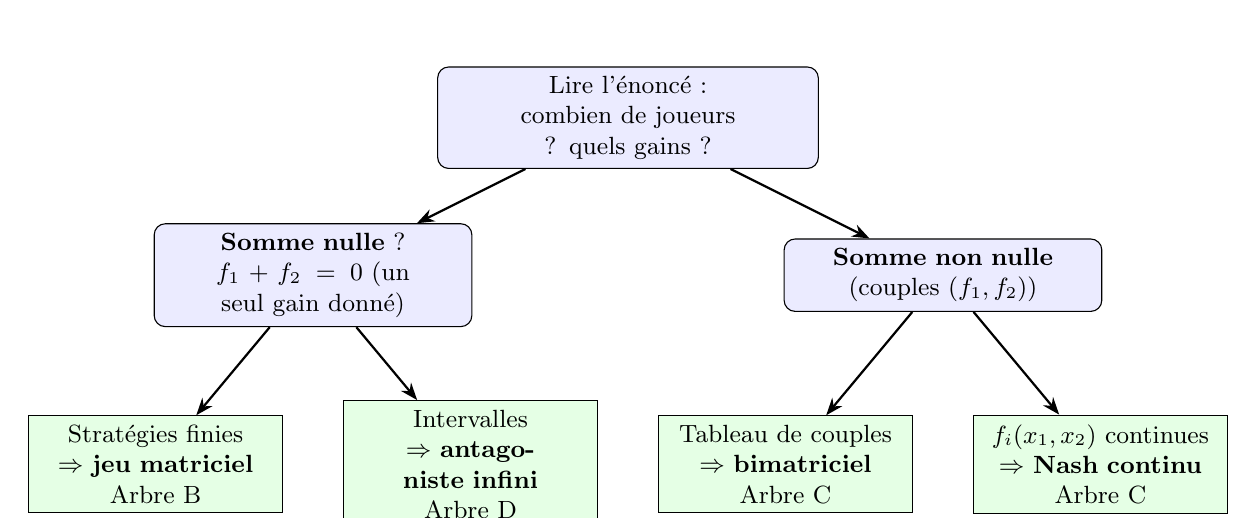
\begin{tikzpicture}[font=\small]
\node[q=4.6cm] (start) at (0,0) {Lire l'énoncé :\\ combien de joueurs ? quels gains ?};
\node[q=3.8cm] (zs) at (-4,-2) {\textbf{Somme nulle} ?\\ $f_1+f_2=0$ (un seul gain donné)};
\node[q=3.8cm] (nzs) at (4,-2) {\textbf{Somme non nulle}\\ (couples $(f_1,f_2)$)};
\node[m=3.0cm] (fin) at (-6,-4.4) {Stratégies finies\\ $\Rightarrow$ \textbf{jeu matriciel}\\ Arbre B};
\node[m=3.0cm] (inf) at (-2,-4.4) {Intervalles\\ $\Rightarrow$ \textbf{antagoniste infini}\\ Arbre D};
\node[m=3.0cm] (bim) at (2,-4.4) {Tableau de couples\\ $\Rightarrow$ \textbf{bimatriciel}\\ Arbre C};
\node[m=3.0cm] (cont) at (6,-4.4) {$f_i(x_1,x_2)$ continues\\ $\Rightarrow$ \textbf{Nash continu}\\ Arbre C};
\draw[arr] (start)--(zs); \draw[arr] (start)--(nzs);
\draw[arr] (zs)--(fin); \draw[arr] (zs)--(inf);
\draw[arr] (nzs)--(bim); \draw[arr] (nzs)--(cont);
\end{tikzpicture}
\end{center}
\textbf{Cas séquentiel} (« joue ensuite », arbre de Kuhn) : forme extensive, résolution par induction à rebours (section~\ref{sec:extensive}).

\subsection{Arbre B : résoudre un jeu matriciel $A$ ($m\times n$)}
\begin{center}
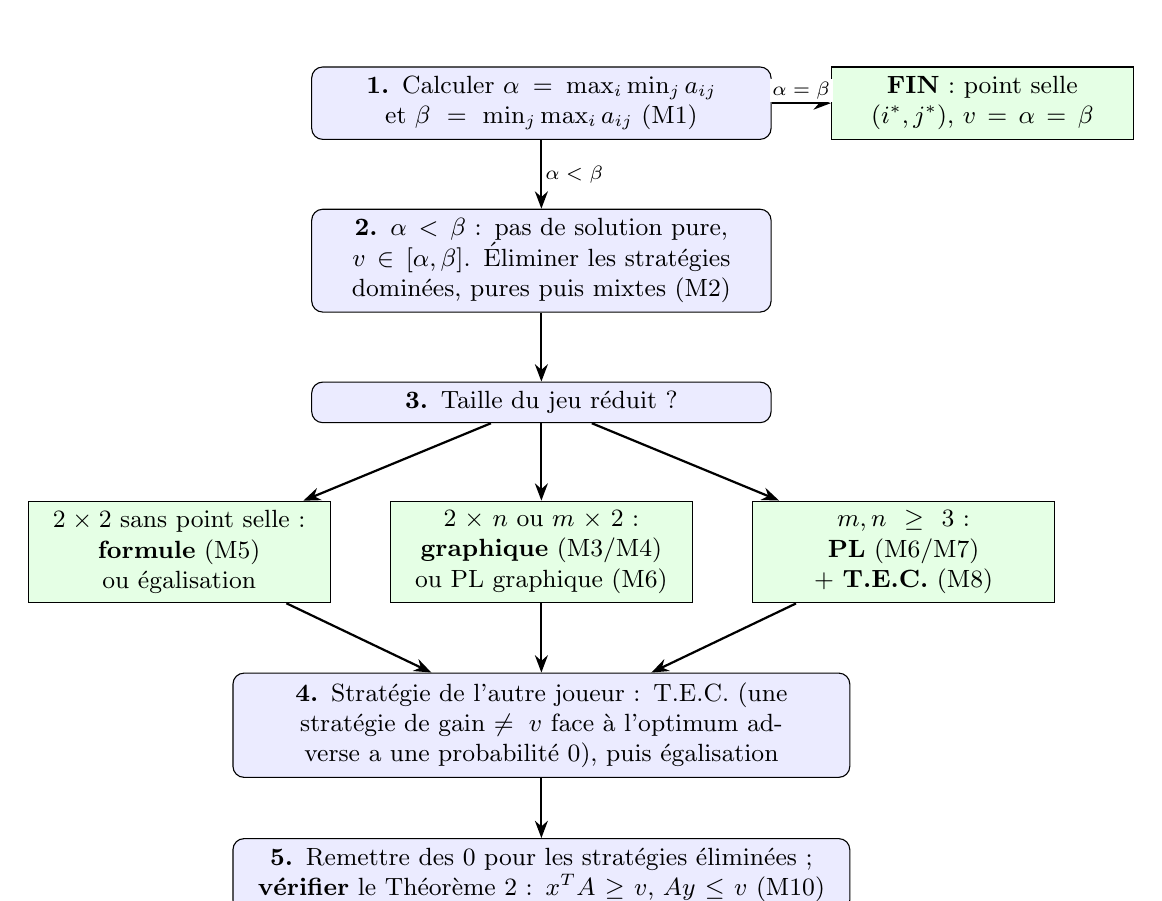
\begin{tikzpicture}[font=\small]
\node[q=5.6cm] (b1) at (0,0) {\textbf{1.} Calculer $\alpha=\max_i\min_j a_{ij}$ et $\beta=\min_j\max_i a_{ij}$ (M1)};
\node[m=3.6cm] (b1y) at (5.6,0) {\textbf{FIN} : point selle $(i^*,j^*)$, $v=\alpha=\beta$};
\node[q=5.6cm] (b2) at (0,-2.0) {\textbf{2.} $\alpha<\beta$ : pas de solution pure, $v\in[\alpha,\beta]$. Éliminer les stratégies dominées, pures puis mixtes (M2)};
\node[q=5.6cm] (b3) at (0,-3.8) {\textbf{3.} Taille du jeu réduit ?};
\node[m=3.6cm] (l1) at (-4.6,-5.7) {$2\times2$ sans point selle :\\ \textbf{formule} (M5)\\ ou égalisation};
\node[m=3.6cm] (l2) at (0,-5.7) {$2\times n$ ou $m\times2$ :\\ \textbf{graphique} (M3/M4)\\ ou PL graphique (M6)};
\node[m=3.6cm] (l3) at (4.6,-5.7) {$m,n\ge3$ :\\ \textbf{PL} (M6/M7)\\ $+$ \textbf{T.E.C.} (M8)};
\node[q=7.6cm] (b4) at (0,-7.9) {\textbf{4.} Stratégie de l'autre joueur : T.E.C. (une stratégie de gain $\ne v$ face à l'optimum adverse a une probabilité 0), puis égalisation};
\node[q=7.6cm] (b5) at (0,-9.8) {\textbf{5.} Remettre des 0 pour les stratégies éliminées ; \textbf{vérifier} le Théorème 2 : $x^TA\ge v$, $Ay\le v$ (M10)};
\draw[arr] (b1)--node[lab,above]{$\alpha=\beta$} (b1y);
\draw[arr] (b1)--node[lab,right]{$\alpha<\beta$} (b2);
\draw[arr] (b2)--(b3);
\draw[arr] (b3)--(l1); \draw[arr] (b3)--(l2); \draw[arr] (b3)--(l3);
\draw[arr] (l1)--(b4); \draw[arr] (l2)--(b4); \draw[arr] (l3)--(b4);
\draw[arr] (b4)--(b5);
\end{tikzpicture}
\end{center}
\textbf{Astuces de l'arbre B :} si des coefficients sont négatifs et que l'on veut la PL du cas $v>0$, ajouter une constante $k$ à toute la matrice (invariance affine, M9) ; si la matrice est un multiple d'une matrice déjà résolue, utiliser M9 directement (ex. $\begin{pmatrix}2&6&0\\4&2&8\end{pmatrix}=2\begin{pmatrix}1&3&0\\2&1&4\end{pmatrix}$).

\subsection{Arbre C : trouver les équilibres de Nash}
\begin{center}
\begin{tikzpicture}[font=\small]
\node[q=4.6cm] (c0) at (0,0) {Jeu non coopératif $\langle X_1,X_2,f_1,f_2\rangle$};
\node[q=4.2cm] (cf) at (-4,-1.6) {$X_i$ finis (tableau de couples)};
\node[q=4.2cm] (cc) at (4,-1.6) {$X_i$ intervalles, $f_i$ dérivables};
\node[m=4.2cm] (cf1) at (-4,-3.4) {\textbf{1.} Élimination itérée des stratégies \textbf{strictement} dominées (N2)};
\node[m=4.2cm] (cf2) at (-4,-5.4) {\textbf{2.} Soulignement des meilleures réponses : cases doublement soulignées $=$ NE purs (N1)};
\node[m=4.2cm] (cf3) at (-4,-7.4) {\textbf{3.} « Tous » les NE d'un $2\times2$ : NE mixte par indifférence (N3)};
\node[m=4.2cm] (cc1) at (4,-3.4) {\textbf{1.} Conditions de Nash : compact convexe, continuité, concavité en $x_i$ (N5)};
\node[m=4.2cm] (cc2) at (4,-5.4) {\textbf{2.} $R_i$ : $\partial f_i/\partial x_i=0$, bords, cas dégénérés (N4)};
\node[m=4.2cm] (cc3) at (4,-7.4) {\textbf{3.} NE $=G_1\cap G_2$ (intersection des graphes) ; tracer les $R_i$};
\node[q=9.5cm] (cend) at (0,-9.5) {\textbf{Toujours :} vérifier qu'aucune déviation unilatérale n'est profitable ; comparer avec Pareto / l'optimum social si demandé (N6)};
\draw[arr] (c0)--(cf); \draw[arr] (c0)--(cc);
\draw[arr] (cf)--(cf1); \draw[arr] (cf1)--(cf2); \draw[arr] (cf2)--(cf3);
\draw[arr] (cc)--(cc1); \draw[arr] (cc1)--(cc2); \draw[arr] (cc2)--(cc3);
\draw[arr] (cf3)--(cend); \draw[arr] (cc3)--(cend);
\end{tikzpicture}
\end{center}

\subsection{Arbre D : jeu antagoniste infini $\langle X,Y,f\rangle$}
\begin{center}
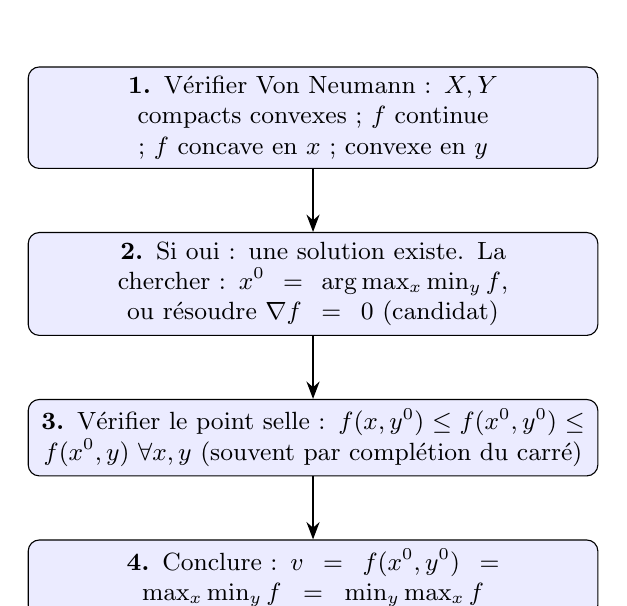
\begin{tikzpicture}[node distance=0.8cm,font=\small]
\node[q=7cm] (d1) {\textbf{1.} Vérifier Von Neumann : $X,Y$ compacts convexes ; $f$ continue ; $f$ concave en $x$ ; convexe en $y$};
\node[q=7cm, below=of d1] (d2) {\textbf{2.} Si oui : une solution existe. La chercher : $x^0=\arg\max_x\min_y f$, ou résoudre $\nabla f=0$ (candidat)};
\node[q=7cm, below=of d2] (d3) {\textbf{3.} Vérifier le point selle : $f(x,y^0)\le f(x^0,y^0)\le f(x^0,y)$ $\forall x,y$ (souvent par complétion du carré)};
\node[q=7cm, below=of d3] (d4) {\textbf{4.} Conclure : $v=f(x^0,y^0)=\max_x\min_y f=\min_y\max_x f$};
\draw[arr] (d1)--(d2); \draw[arr] (d2)--(d3); \draw[arr] (d3)--(d4);
\end{tikzpicture}
\end{center}

%=====================================================================
\section{Notions de base (Chapitre 1, pages 1--5)}

\begin{propbox}{Définitions fondamentales}
\begin{itemize}[leftmargin=*]
\item \textbf{Jeu} : toute interaction entre agents (\emph{joueurs}) qui font des choix parmi des actions possibles, dans un cadre fixé à l'avance (\emph{règles du jeu}). La théorie des jeux étudie les situations de \emph{conflit} où des individus font des choix en interaction.
\item \textbf{Joueur} : l'unité de décision. \textbf{Stratégie} : un choix parmi toutes les actions possibles d'un joueur. \textbf{Issue} : le résultat des choix de \emph{tous} les joueurs ; on lui associe un gain pour chacun.
\item \textbf{Jeu non coopératif} : les joueurs ne forment pas de coalition et ne contractent pas d'accords contraignants ; chacun maximise son propre gain.
\item \textbf{Forme normale} $J=\langle I,X,f\rangle$ : $I=\{1,\dots,n\}$ joueurs, $X=X_1\times\dots\times X_n$ ensemble des issues, $x_i\in X_i$ stratégie de $i$, $f=(f_1,\dots,f_n)$, $f_i:X\to\mathbb{R}$ gain de $i$. Les joueurs jouent \textbf{simultanément}, en \textbf{un seul coup}.
\item \textbf{Jeu à deux personnes à somme nulle} (\textbf{antagoniste}) : $I=\{1,2\}$ et $f_1(x,y)+f_2(x,y)=0$. On ne donne que $f=f_1$ (gain de 1 $=$ perte de 2). Chacun connaît $X,Y,f$ mais ignore le choix de l'autre.
\item \textbf{Jeu matriciel} : jeu antagoniste où les ensembles de stratégies sont finis : $X=\{1,\dots,m\}$ (lignes, joueur 1), $Y=\{1,\dots,n\}$ (colonnes, joueur 2), $f(i,j)=a_{ij}$. Le joueur 1 reçoit $a_{ij}$, le joueur 2 reçoit $-a_{ij}$.
\end{itemize}
\end{propbox}

%=====================================================================
\section{Jeux matriciels en stratégies pures (pages 5--8)}

\begin{propbox}{Valeurs inférieure et supérieure}
\[
\alpha=\max_{1\le i\le m}\ \min_{1\le j\le n}a_{ij}\quad(\text{\textbf{valeur inférieure}, maximin, gain minimum garanti du joueur 1}),
\]
\[
\beta=\min_{1\le j\le n}\ \max_{1\le i\le m}a_{ij}\quad(\text{\textbf{valeur supérieure}, minimax, perte maximale du joueur 2}).
\]
On a toujours $\alpha\le\beta$. \textbf{Définition :} le jeu admet une solution $(i^*,j^*)$ ssi $\alpha=\beta=a_{i^*j^*}$. $(i^*,j^*)$ est un \textbf{point selle} et $v=a_{i^*j^*}$ la \textbf{valeur du jeu}.
\end{propbox}

\begin{propbox}{Propriétés du point selle (page 8)}
\begin{enumerate}[leftmargin=*]
\item $a_{ij^*}\le a_{i^*j^*}\le a_{i^*j}$ pour tous $i,j$ : $a_{i^*j^*}$ est \textbf{minimal dans sa ligne et maximal dans sa colonne}.
\item Deux points selle ont la même valeur : $a_{i^*j^*}=a_{i^1j^1}$.
\item \textbf{Interchangeabilité} : si $(i^*,j^*)$ et $(i^1,j^1)$ sont des points selle, alors $(i^*,j^1)$ et $(i^1,j^*)$ aussi.
\end{enumerate}
\textbf{Signification} : si un joueur joue sa stratégie de point selle, l'autre ne peut pas améliorer son gain en déviant.
\end{propbox}

\textbf{Exemple du cours :} $A=\begin{pmatrix}5&3&4&3\\7&2&0&-2\\0&-1&-4&2\end{pmatrix}$ : minima des lignes $3,-2,-4$, $\alpha=3$ ; maxima des colonnes $7,3,4,3$, $\beta=3$. Points selle $(1,2)$ et $(1,4)$, $v=3$.

%=====================================================================
\section{Stratégies mixtes (pages 9--12)}

\begin{propbox}{Extension mixte}
Si $\alpha<\beta$, chaque joueur choisit sa stratégie au hasard :
\[
\Xt=\Big\{x\in\mathbb{R}^m: x_i\ge0,\ \sum_{i=1}^m x_i=1\Big\},\qquad \Yt=\Big\{y\in\mathbb{R}^n: y_j\ge0,\ \sum_{j=1}^n y_j=1\Big\},
\]
\[
E(x,y)=\sum_{i=1}^m\sum_{j=1}^n a_{ij}x_iy_j=x^TAy\qquad(\text{gain moyen}).
\]
$\tilde J=\langle I=\{1,2\},\Xt,\Yt,E\rangle$ est l'\textbf{extension mixte} (jeu élargi). J1 maximise $E$, J2 minimise $E$. Une stratégie pure est le vecteur $e_i=(0,\dots,1,\dots,0)$.

Utiles : $x^TA=\big(\sum_i a_{ij}x_i\big)_j$ (gain de J1 contre chaque colonne pure) ; $Ay=\big(\sum_j a_{ij}y_j\big)_i$ (gain de J1 avec chaque ligne pure contre $y$).
\end{propbox}

\begin{propbox}{Théorème d'existence 1 (minimax de Von Neumann)}
Pour tout jeu matriciel, $\tilde\alpha=\max_{x\in\Xt}\min_{y\in\Yt}E(x,y)$ et $\tilde\beta=\min_{y\in\Yt}\max_{x\in\Xt}E(x,y)$ existent et sont égaux : \textbf{tout jeu matriciel admet une solution en stratégies mixtes}. On a $\alpha\le v\le\beta$.
\end{propbox}

\begin{propbox}{Théorème 2 (caractérisation des solutions)}
$x^0\in\Xt$, $y^0\in\Yt$ sont solution de $\tilde J$ de valeur $v$ si et seulement si
\[
\sum_{i=1}^m a_{ij}x^0_i\ge v\ \ (j=1..n),\qquad \sum_{j=1}^n a_{ij}y^0_j\le v\ \ (i=1..m),\qquad x^0,y^0\ \text{distributions de probabilité}.
\]
Équivalent : $E(x,y^0)\le E(x^0,y^0)=v\le E(x^0,y)$ pour tous $x,y$ (\textbf{point selle} de $E$).
\end{propbox}

\begin{propbox}{Conséquences (TD1 Ex.~5 ; cours p.~29--30)}
Si $(x,y)$ est solution de valeur $v$, alors $E(x,y)=v$ et
\[
\sum_j a_{i_0j}y_j<v\ \Rightarrow\ x_{i_0}=0,\qquad \sum_i a_{ij_0}x_i>v\ \Rightarrow\ y_{j_0}=0,
\]
et réciproquement $x_{i_0}>0\Rightarrow\sum_j a_{i_0j}y_j=v$, $y_{j_0}>0\Rightarrow\sum_i a_{ij_0}x_i=v$.

\emph{Preuve en une ligne :} $\sum_i x_i(v-(Ay)_i)=v-E(x,y)=0$ est une somme de termes $\ge0$, donc chaque terme est nul.
\end{propbox}

%=====================================================================
\section{Domination (pages 18--23)}

\begin{propbox}{Définitions}
\textbf{Joueur 1 (maximise, compare des lignes)} : $i^*$ est \textbf{dominée} par $\bar i$ si $a_{i^*j}\le a_{\bar ij}$ pour tout $j$, avec au moins une inégalité stricte ; \textbf{strictement dominée} si toutes sont strictes. $i^*$ est \textbf{dominante} si elle domine toutes les autres.

\textbf{Joueur 2 (minimise, compare des colonnes)} : $j^*$ est dominée par $\bar j$ si $a_{ij^*}\ge a_{i\bar j}$ pour tout $i$ (au moins une stricte). \emph{Le sens est inversé !}

\textbf{Dans l'extension mixte} : $e_{i_0}$ est dominée s'il existe $p\in\Xt$ avec $p_{i_0}=0$ et $L_{i_0}\le\sum_i p_iL_i$ (strictement dominée si $<$ partout) ; pour J2, $C_{j_0}\ge\sum_j q_jC_j$ avec $q_{j_0}=0$.
\end{propbox}

\begin{propbox}{Propositions (page 19, 22)}
\begin{enumerate}[leftmargin=*]
\item Le gain garanti optimal d'un joueur est inchangé quand on retire ses stratégies dominées.
\item Le jeu réduit a la \textbf{même valeur} que le jeu initial.
\item Une solution du jeu réduit (complétée par des 0) est une solution du jeu initial.
\item On peut \textbf{perdre des solutions} (points selle) mais jamais l'\textbf{existence} d'une solution.
\item Si $i_0$ est strictement dominée dans l'extension mixte, alors $p_{i_0}=0$ dans toute solution.
\end{enumerate}
\end{propbox}

\begin{rembox}{Conséquence pratique (DM2 Ex.~1)}
Éliminer une stratégie \emph{strictement} dominée ne perd aucune solution. Éliminer une stratégie \emph{faiblement} (largement) dominée peut en perdre : dans le DM2, l'élimination de $C_1$ ne laisse que $y=(0,1)$, alors que toutes les $y=(t,1-t)$, $t\in[0,\frac89]$, sont optimales. Si l'on demande « toutes les solutions » ou « la solution est-elle unique ? », travailler sur le jeu \emph{initial}.
\end{rembox}

%=====================================================================
\section{Fiches méthodes : jeux matriciels}\label{sec:methodes}

\begin{methbox}{M1 -- Recherche d'un point selle (stratégies pures)}
\begin{enumerate}[leftmargin=*]
\item Écrire le minimum de chaque ligne à droite ; $\alpha=$ le plus grand.
\item Écrire le maximum de chaque colonne en bas ; $\beta=$ le plus petit.
\item Si $\alpha=\beta$ : tous les $a_{ij}$ égaux à cette valeur, minimaux dans leur ligne et maximaux dans leur colonne, sont des points selle. Sinon : pas de solution pure, $v\in[\alpha,\beta]$.
\end{enumerate}
\textbf{Exemples :} TD1 Ex.~1 ($\alpha=\beta=1$, point selle $(2,1)$) ; DM2 ($\alpha=\beta=\frac16$, point selle $(3,2)$) ; DM1/Examen $J$ ($\alpha=1<2=\beta$).
\end{methbox}
\begin{whenbox}
Toujours en \textbf{première} étape, quelle que soit la question. Elle donne aussi l'encadrement $\alpha\le v\le\beta$ (et le signe de $v$ pour la PL).
\end{whenbox}

\begin{methbox}{M2 -- Élimination des stratégies dominées}
\begin{enumerate}[leftmargin=*]
\item \textbf{J1, lignes} : chercher $L_k\le L_l$ composante par composante (la plus petite est éliminée).
\item \textbf{J2, colonnes} : chercher $C_k\ge C_l$ (la plus grande est éliminée, J2 minimise).
\item \textbf{Mixte} : pour $L_{i_0}$, poser $\lambda L_a+(1-\lambda)L_b>L_{i_0}$, écrire une inégalité par colonne, intersecter les intervalles de $\lambda$, \textbf{exhiber une valeur} (par ex. $\lambda=\frac23$) et \textbf{vérifier numériquement}. Choisir pour $L_a,L_b$ les lignes qui « couvrent » chacune un point faible de $L_{i_0}$.
\item Itérer (une élimination peut en créer d'autres). Garder la trace des stratégies supprimées pour remettre des 0 à la fin.
\end{enumerate}
\textbf{Exemple type (DM1 / Examen $J'$) :} $L_3\le L_2$ (large) ; $L_4<\lambda L_1+(1-\lambda)L_2$ pour $\lambda\in\,]\frac12,\frac34[$ ; puis $C_3>\mu C_1+(1-\mu)C_2$ pour $\mu\in\,]\frac14,\frac12[$.
\end{methbox}
\begin{whenbox}
Juste après M1 si $\alpha<\beta$, ou quand l'énoncé le demande. Pour montrer qu'une stratégie n'est \emph{pas} dominée, trouver une colonne (ou une ligne) qui rend le système impossible.
\end{whenbox}

\begin{methbox}{M3 -- Méthode graphique pour un jeu $2\times n$ (joueur 1)}
\begin{enumerate}[leftmargin=*]
\item Poser $x=(p,1-p)$. Pour chaque colonne $j$ : $g_j(p)=a_{1j}p+a_{2j}(1-p)$ (droite).
\item Tracer les $n$ droites sur $[0,1]$ ; $\varphi(p)=\min_j g_j(p)$ est l'\textbf{enveloppe inférieure} (concave, affine par morceaux).
\item $v=\max_p\varphi(p)$ : au sommet de l'enveloppe, intersection d'une droite croissante et d'une droite décroissante. Résoudre $g_k(p)=g_l(p)$.
\item Vérifier que les autres droites passent \textbf{au-dessus} de $v$ en $p^*$ : les colonnes correspondantes ont $y_j=0$.
\item Joueur 2 : jouer uniquement $C_k,C_l$ ; $y=(q,1-q)$ sur ces colonnes, égaliser les gains des deux lignes.
\end{enumerate}
\textbf{Exemples :} DM1 ($p=\frac13$, $v=\frac53$), TD1 Ex.~2 ($v=\frac{10}3$), TD1 Ex.~4 ($p=\frac9{11}$, $v=\frac{42}{11}$, colonnes actives $C_4,C_5$).
\end{methbox}

\begin{methbox}{M4 -- Méthode graphique pour un jeu $m\times 2$ (joueur 2)}
$y=(q,1-q)$ ; pour chaque ligne $i$ : $h_i(q)=a_{i1}q+a_{i2}(1-q)$. Tracer l'\textbf{enveloppe supérieure} $\max_i h_i(q)$ ; $v$ est son \textbf{minimum}. Les lignes qui passent en dessous de $v$ ont $x_i=0$.
\end{methbox}

\begin{methbox}{M5 -- Formule fermée pour un jeu $2\times2$ \textbf{sans point selle}}
$A=\begin{pmatrix}a&b\\c&d\end{pmatrix}$, $D=a+d-b-c\ne0$ :
\[
x_1=\frac{d-c}{D},\quad x_2=\frac{a-b}{D},\qquad y_1=\frac{d-b}{D},\quad y_2=\frac{a-c}{D},\qquad v=\frac{ad-bc}{D}.
\]
\emph{Origine :} égalisation $E(x,C_1)=E(x,C_2)$ et $E(L_1,y)=E(L_2,y)$. \textbf{À n'utiliser qu'après avoir vérifié $\alpha<\beta$} ; sinon on obtient des « probabilités » hors de $[0,1]$.
\textbf{Exemple :} $\begin{pmatrix}3&-2\\-1&3\end{pmatrix}$ (cours p.~20, après élimination) : $D=9$, $x=(\frac49,\frac59)$, $y=(\frac59,\frac49)$, $v=\frac79$.
\end{methbox}

\begin{methbox}{M6 -- Programmation linéaire, cas $v>0$ (pages 13--15)}
Condition : $v>0$. Elle est garantie dès que $\alpha>0$ (au moins une ligne à coefficients tous strictement positifs), en particulier si tous les $a_{ij}>0$.
\begin{enumerate}[leftmargin=*]
\item Poser $p_i=\frac{x_i}{v}$, $q_j=\frac{y_j}{v}$ ; alors $\sum p_i=\sum q_j=\frac1v$.
\item \textbf{Primal (joueur 1)} : J1 maximise $v\iff$ minimise $\frac1v$ :
\[
(III)\quad \min\sum_{i=1}^m p_i\quad\text{s.c.}\quad \sum_{i=1}^m a_{ij}p_i\ge1\ (j=1..n),\quad p_i\ge0.
\]
\item \textbf{Dual (joueur 2)} :
\[
(IV)\quad \max\sum_{j=1}^n q_j\quad\text{s.c.}\quad \sum_{j=1}^n a_{ij}q_j\le1\ (i=1..m),\quad q_j\ge0.
\]
\item Résoudre l'un (graphiquement s'il a 2 variables, sinon simplexe), puis :
\[
v=\frac1{\sum p_i}=\frac1{\sum q_j},\qquad x_i=p_iv,\qquad y_j=q_jv.
\]
\end{enumerate}
\textbf{Résolution graphique de $(III)$ à 2 variables :} tracer les droites $\Delta_j:\ a_{1j}p_1+a_{2j}p_2=1$, région admissible \emph{au-dessus} de toutes, lister les sommets de sa frontière, évaluer $p_1+p_2$ en chaque sommet ; le plus petit est l'optimum.
\textbf{Exemples :} DM1 : $(p_1,p_2)=(\frac15,\frac25)$, $v=\frac53$. TD1 Ex.~4 : sommets $(0,1)$, $(\frac1{13},\frac3{13})$, $(\frac3{14},\frac1{21})$, $(\frac12,0)$ ; optimum $(\frac3{14},\frac1{21})$, $v=\frac{42}{11}$.
\end{methbox}

\begin{methbox}{M7 -- Programmation linéaire, cas $v$ quelconque (pages 16--17)}
\textbf{Méthode du cours :} variables d'écart $x_{m+j}\ge0$ : $\sum_ia_{ij}x_i-x_{m+j}=v$, puis soustraire la première égalité des autres pour éliminer $v$ :
\[
\max\ \sum_i a_{i1}x_i-x_{m+1}\quad\text{s.c.}\quad \sum_i(a_{ij}-a_{i1})x_i-x_{m+j}+x_{m+1}=0\ (j=2..n),\quad \sum_ix_i=1,\ x\ge0.
\]
\textbf{Méthode pratique (recommandée) :} ajouter une constante $k$ telle que $a_{ij}+k>0$ pour tout $(i,j)$, résoudre par M6, puis $v(A)=v(A+k)-k$ ; les stratégies optimales ne changent pas (M9).
\end{methbox}

\begin{methbox}{M8 -- Théorème des écarts complémentaires (T.E.C.)}
Pour $(III)$/$(IV)$ optimaux :
\[
p_i>0\ \Rightarrow\ \sum_j a_{ij}q_j=1,\qquad \sum_i a_{ij}p_i>1\ \Rightarrow\ q_j=0
\]
(et symétriquement $q_j>0\Rightarrow$ contrainte $j$ de $(III)$ saturée). \textbf{Usage :} après avoir résolu le primal, repérer les contraintes non saturées ($\Rightarrow q_j=0$) et les $p_i>0$ ($\Rightarrow$ égalités) ; résoudre le petit système obtenu.
\textbf{Exemple (cours p.~29) :} $p=(\frac15,\frac25)$, $4p_2=\frac85>1\Rightarrow q_3=0$ ; $q_1+3q_2=1$, $2q_1+q_2=1\Rightarrow q=(\frac25,\frac15,0)$, $y=(\frac23,\frac13,0)$.
\textbf{Interprétation jeu :} une colonne qui coûte plus que $v$ à J2 face à $x^*$ n'est jamais jouée ; une ligne qui rapporte moins que $v$ à J1 face à $y^*$ n'est jamais jouée.
\end{methbox}

\begin{methbox}{M9 -- Invariance par transformation affine (DM1 Ex.~2)}
Si $b_{ij}=\alpha a_{ij}+\beta$ avec $\alpha>0$ : $E_B=\alpha E_A+\beta$ (car $\sum_{i,j}x_iy_j=1$), donc
\[
\text{mêmes solutions optimales}\qquad\text{et}\qquad v_B=\alpha v_A+\beta.
\]
Preuve : l'application $t\mapsto\alpha t+\beta$ est strictement croissante, elle conserve les inégalités du point selle. \textbf{Si $\alpha<0$} : les inégalités s'inversent, les rôles max/min s'échangent ; le résultat est faux.
\textbf{Usages :} rendre la matrice positive pour M6 ; simplifier les fractions (multiplier par un dénominateur commun, ex. DM2 $\times12$) ; reconnaître un multiple d'un jeu déjà résolu.
\end{methbox}

\begin{methbox}{M10 -- Vérification finale (à écrire sur la copie)}
Calculer $x^{*T}A$ (vecteur ligne) et $Ay^*$ (vecteur colonne). Il faut $x^{*T}A\ge v$ \emph{composante par composante} et $Ay^*\le v$. Les composantes égales à $v$ correspondent aux stratégies actives ; une composante $\ne v$ doit correspondre à une probabilité nulle chez l'adversaire.
\textbf{Exemple (DM1 $J'$) :} $x^{*T}A'=(\frac{10}3,\frac{10}3,\frac{11}3,\frac{16}3)$, $A'y^*=(\frac{10}3,\frac{10}3,\frac{10}3,\frac83)^T$.
\end{methbox}

%=====================================================================
\section{Jeux antagonistes infinis (Chapitre 2, pages 1--3)}

\begin{propbox}{Définitions et théorèmes}
$J=\langle I,X,Y,f\rangle$ avec $X,Y$ \textbf{infinis} (souvent des intervalles), $f:X\times Y\to\mathbb{R}$ gain du joueur 1.
\begin{itemize}[leftmargin=*]
\item \textbf{Théorème 1} : $x^0,y^0$ sont optimales $\iff(x^0,y^0)$ est un point selle de $f$ : $f(x,y^0)\le f(x^0,y^0)\le f(x^0,y)$, $\forall x\in X,\forall y\in Y$.
\item \textbf{Théorème 2} : $(x^0,y^0)$ solution $\iff\max_x\min_y f=\min_y\max_x f=f(x^0,y^0)$, la \textbf{valeur} du jeu. $\alpha=\max_x\min_yf$ est la valeur inférieure, $\beta=\min_y\max_xf$ la valeur supérieure.
\item \textbf{Théorème de Von Neumann} : si (1) $X,Y$ compacts convexes, (2) $f$ continue sur $X\times Y$, (3) $x\mapsto f(x,y)$ concave $\forall y$, (4) $y\mapsto f(x,y)$ convexe $\forall x$, alors le jeu admet au moins une solution.
\end{itemize}
\end{propbox}

\begin{methbox}{M11 -- Vérifier Von Neumann et trouver le point selle}
\begin{enumerate}[leftmargin=*]
\item Compact : fermé et borné (dans $\mathbb{R}$ : intervalle $[a,b]$). Convexe : intervalle. \emph{Contre-exemple :} $\mathbb{R}$ ou $[0,+\infty[$ ne sont pas compacts.
\item Continuité : polynômes, sommes, produits de fonctions continues.
\item Concavité en $x$ : $\frac{\partial^2f}{\partial x^2}\le0$ ; convexité en $y$ : $\frac{\partial^2f}{\partial y^2}\ge0$ (une fonction affine est à la fois concave et convexe).
\item Candidat : $\frac{\partial f}{\partial x}=0$, $\frac{\partial f}{\partial y}=0$ (ou un bord). Vérifier par la définition du point selle, en complétant le carré.
\end{enumerate}
\textbf{Exemple (cours, TD1 Ex.~3)} : $f=y^2-x^2$ sur $[-1,1]^2$ : $f(x,0)=-x^2\le0=f(0,0)\le y^2=f(0,y)$ ; point selle $(0,0)$, $v=0$.
\end{methbox}

%=====================================================================
\section{Jeux non coopératifs et équilibre de Nash}\label{sec:nash}

\begin{propbox}{Définitions (Chapitre 2, pages 3--7 ; DM2)}
\begin{itemize}[leftmargin=*]
\item Notation : $(t_i,x_{I-i})=(x_1,\dots,x_{i-1},t_i,x_{i+1},\dots,x_n)$.
\item \textbf{Équilibre de Nash} : $x^*$ tel que $\forall i,\ \forall x_i\in X_i,\ f_i(x_i,x^*_{I-i})\le f_i(x_i^*,x^*_{I-i})$. \emph{Aucun joueur ne peut augmenter \textbf{strictement} son gain en déviant seul.}
\item \textbf{Meilleure réponse} : $R_i(x_{I-i})=\arg\max_{x_i\in X_i}f_i(x_i,x_{I-i})$ (un ensemble).
\item \textbf{Caractérisations} : $x^*$ NE $\iff x^*\in R(x^*)$ (\textbf{point fixe} de $R=(R_1,R_2)$) $\iff x^*\in G_1\cap G_2$ (\textbf{intersection des graphes} des meilleures réponses).
\item \textbf{Stratégie strictement dominante} : $f_i(x_i^*,x_{I-i})>f_i(x_i,x_{I-i})$ pour tout $x_i\ne x_i^*$ et tout $x_{I-i}$ ; équivalent : $R_i\equiv\{x_i^*\}$ constante.
\item \textbf{Optimum de Pareto} : issue telle qu'aucune autre n'augmente le gain d'un joueur sans diminuer celui d'un autre. \textbf{Optimum social} : issue maximisant $\sum_if_i$.
\end{itemize}
\end{propbox}

\begin{propbox}{Lien zéro-somme / Nash}
Pour un jeu à somme nulle, $(x^*,y^*)$ est un équilibre de Nash (avec $f_1=f$, $f_2=-f$) si et seulement si c'est un point selle. Un point selle est donc un cas particulier d'équilibre de Nash.
\end{propbox}

\begin{methbox}{N1 -- Équilibres purs d'un jeu bimatriciel (soulignement)}
\begin{enumerate}[leftmargin=*]
\item Pour chaque \textbf{colonne}, souligner le plus grand \textbf{premier} nombre (meilleure réponse de J1).
\item Pour chaque \textbf{ligne}, souligner le plus grand \textbf{second} nombre (meilleure réponse de J2).
\item Les cases dont les deux nombres sont soulignés sont les NE purs. Rédaction : pour chaque case candidate, écrire les déviations et leurs gains.
\end{enumerate}
\textbf{Exemple (cours p.~6)} : $\begin{pmatrix}(8,8)&(4,7)&(10,6)\\(9,2)&(5,5)&(6,3)\end{pmatrix}$, unique NE $(t_2,s_2)$, gains $(5,5)$, alors que $(t_1,s_1)$ donnerait $(8,8)$ (coordination impossible sans communication).
\end{methbox}

\begin{methbox}{N2 -- Élimination itérée des stratégies strictement dominées}
J1 compare les \textbf{premiers} nombres ligne à ligne ; J2 les \textbf{seconds} nombres colonne à colonne (les deux maximisent). Éliminer, recommencer. S'il reste une seule issue, c'est l'unique NE.
\textbf{Exemples :} cours p.~7 ($s_3$ dominée par $s_2$, puis $t_1$ par $t_2$, puis il reste $(t_2,s_2)$) ; prairie commune TD2 Ex.~3 (« 2 vaches » strictement dominante, NE $(2,2)$, dilemme du prisonnier).
\end{methbox}

\begin{methbox}{N3 -- Équilibre mixte d'un jeu $2\times2$ (principe d'indifférence)}
La probabilité $q$ de J2 rend \textbf{J1} indifférent entre ses deux lignes : $a_{11}q+a_{12}(1-q)=a_{21}q+a_{22}(1-q)$ (gains de J1). La probabilité $p$ de J1 rend \textbf{J2} indifférent entre ses deux colonnes (gains de J2).
\textbf{Exemples :} chasse au cerf $p=q=\frac79$ (gain $\frac{70}9$) ; chicken $p=q=\frac12$ (gain $-\frac12$). Un jeu $2\times2$ « de coordination » ou « chicken » a 2 NE purs et 1 NE mixte.
\end{methbox}

\begin{methbox}{N4 -- Meilleures réponses dans un jeu continu}
\begin{enumerate}[leftmargin=*]
\item Fixer $x_{-i}$, étudier $\varphi(x_i)=f_i(x_i,x_{-i})$. Si $\varphi''<0$ : unique maximum, en $\varphi'=0$ si ce point est dans $X_i$, \textbf{sinon au bord} le plus proche (projection).
\item \textbf{Cas dégénérés} : si $\varphi$ est constante (ex. DM2 : $x_2=0\Rightarrow f_1\equiv0$), $R_i=X_i$ tout entier.
\item Écrire $R_i$ \emph{par morceaux} avec ses conditions (Cournot : $R_1(x_2)=\max(0,\frac{p-x_2}2)$).
\item Résoudre $x_1\in R_1(x_2)$, $x_2\in R_2(x_1)$ ; examiner séparément les morceaux de bord.
\item Vérifier par complétion du carré : $f_1(x_1,x_2^*)=f_1^*-c(x_1-x_1^*)^2\le f_1^*$.
\end{enumerate}
\textbf{Exemples :} TD2 Ex.~4 / Examen Ex.~2 ($R_1(x_2)=x_2$, NE $=$ diagonale) ; Cournot ($\frac p3,\frac p3$) ; DM2 ($R_1=\frac1{2x_2}$, $R_2=\frac12$, NE $(1,\frac12)$).
\end{methbox}

\begin{methbox}{N5 -- Théorème d'existence de Nash (conditions à vérifier)}
Pour tout $i$ : $X_i$ \textbf{compact, convexe, non vide} ; $f_i$ \textbf{continue} sur $X$ ; $x_i\mapsto f_i(x_i,x_{-i})$ \textbf{concave} (ou quasi-concave). Alors il existe au moins un équilibre de Nash. Même plan de rédaction que Von Neumann, \textbf{mais} la concavité porte sur \emph{chaque joueur par rapport à sa propre variable}. \emph{Remarque :} si $X_i=\mathbb{R}$ (DM2), le théorème ne s'applique pas (non compact), ce qui n'empêche pas un NE d'exister.
\end{methbox}

\begin{methbox}{N6 -- Optimum social, Pareto et contrat avec sanction}
\begin{enumerate}[leftmargin=*]
\item Tableau des sommes $f_1+f_2$ ; maximum $=$ optimum social.
\item Pareto : éliminer toute issue dominée composante par composante par une autre.
\item Contrat « jouer $s$ » avec sanction $S$ sur la déviation : retrancher $S$ aux gains de la stratégie interdite ; exiger que la déviation ne soit plus profitable ($\Rightarrow$ seuil sur $S$, inégalité \textbf{stricte} pour un équilibre unique).
\end{enumerate}
\textbf{Exemple (prairie)} : optimum $(1,1)$, $(5,5)$ ; $S>1$ rend $(1,1)$ unique NE, $S>2$ rend « 1 vache » strictement dominante.
\end{methbox}

\begin{rembox}{Jeux classiques à reconnaître}
\begin{tabular}{p{3.2cm}p{11cm}}
\textbf{Dilemme du prisonnier} & Stratégie strictement dominante pour chacun, NE unique non Pareto-optimal (prairie commune, Cournot). \\
\textbf{Chasse au cerf} & Coordination : 2 NE purs (l'un Pareto-dominant, l'autre « prudent ») et 1 NE mixte. \\
\textbf{Poule mouillée (chicken)} & 2 NE purs asymétriques, 1 NE mixte symétrique, pas de stratégie dominée. \\
\textbf{Cournot} & Jeu continu : $R_i$ affines décroissantes, NE à leur intersection $(\frac p3,\frac p3)$.
\end{tabular}
\end{rembox}

%=====================================================================
\section{Forme extensive (Chapitre 1, pages 32--33)}\label{sec:extensive}
Représentation par un \textbf{arbre} (arbre de Kuhn) : chaque nœud est un joueur qui décide, chaque branche une action, chaque feuille une issue avec les gains. Elle convient aux jeux \textbf{séquentiels}. \textbf{Complément de méthode} (induction à rebours) : en partant des feuilles, chaque joueur choisit sa meilleure branche ; on remonte jusqu'à la racine.

\textbf{Exemple du cours (systèmes MAC/CAM)} : J1 joue puis J2. Gains : (MAC,MAC) $=(200,600)$, (MAC,CAM) $=(100,100)$, (CAM,MAC) $=(100,100)$, (CAM,CAM) $=(600,200)$. J2 suit toujours J1 (600 $>$ 100 ; 200 $>$ 100), donc J1 compare 200 et 600 et choisit CAM. Issue : (CAM,CAM), gains $(600,200)$.

%=====================================================================
\section{Formulaire}\label{sec:formulaire}
\begin{center}
\renewcommand{\arraystretch}{1.5}
\begin{tabular}{|p{4.2cm}|p{10.8cm}|}
\hline
Valeurs pures & $\alpha=\max_i\min_ja_{ij}\le\beta=\min_j\max_ia_{ij}$ ; point selle $\iff\alpha=\beta$\\\hline
Gain mixte & $E(x,y)=x^TAy=\sum_{i,j}a_{ij}x_iy_j$\\\hline
Encadrement & $\alpha\le v\le\beta$ ; $v$ existe toujours (minimax)\\\hline
Théorème 2 & $x^TA\ge v\mathbf 1^T$, $Ay\le v\mathbf 1$\\\hline
$2\times2$ sans selle & $D=a+d-b-c$, $x_1=\frac{d-c}D$, $y_1=\frac{d-b}D$, $v=\frac{ad-bc}D$\\\hline
PL ($v>0$) & $p=\frac xv$ : $\min\sum p_i$, $A^Tp\ge\mathbf 1$ ; $q=\frac yv$ : $\max\sum q_j$, $Aq\le\mathbf 1$ ; $v=\frac1{\sum p_i}$\\\hline
T.E.C. & $p_i>0\Rightarrow(Aq)_i=1$ ; $(A^Tp)_j>1\Rightarrow q_j=0$\\\hline
Affine & $B=\alpha A+\beta$, $\alpha>0$ : mêmes solutions, $v_B=\alpha v_A+\beta$\\\hline
Domination J1 & ligne $L_k\le L_l$ ; J2 : colonne $C_k\ge C_l$ (sens inversé)\\\hline
Nash & $f_i(x_i,x^*_{-i})\le f_i(x^*)$ $\forall i,x_i$ ; $\mathcal E=G_1\cap G_2$ ; point fixe de $R$\\\hline
Indifférence $2\times2$ & $q$ (de J2) égalise les gains de J1 ; $p$ (de J1) égalise ceux de J2\\\hline
Von Neumann / Nash & compact convexe $+$ continue $+$ concave en sa variable (et convexe en $y$ pour VN)\\\hline
\end{tabular}
\end{center}

%=====================================================================
\section{Pièges classiques}\label{sec:pieges}
\begin{piegebox}
\begin{enumerate}[leftmargin=*]
\item \textbf{Sens de la domination pour J2} : J2 minimise, une colonne est dominée si elle est \emph{plus grande}.
\item \textbf{Large vs stricte} : préciser toujours. $L_3=(4,2,2,6)\le L_2=(4,2,3,8)$ est large (égalités). Une stratégie mixte peut dominer strictement là où aucune pure ne le fait.
\item \textbf{Élimination faible} : peut faire perdre des solutions (DM2). Pour l'unicité, revenir au jeu initial.
\item \textbf{Formule $2\times2$} utilisée alors qu'il y a un point selle : résultat absurde. Toujours M1 d'abord.
\item \textbf{PL avec $v\le0$} : le changement $p=x/v$ n'a plus de sens. Translater la matrice (M9) ou utiliser M7.
\item \textbf{Oublier de remettre les zéros} pour les stratégies éliminées dans la solution du jeu initial.
\item \textbf{Gain du joueur 2} : c'est $-v$ (sa perte vaut $v$).
\item \textbf{Méthode graphique} : J1 prend le \emph{maximum de l'enveloppe inférieure} ; J2 le \emph{minimum de l'enveloppe supérieure}. Vérifier que les droites non utilisées sont du bon côté de $v$.
\item \textbf{PL graphique} : la frontière de la région admissible change de contrainte active ; lister \emph{tous} les sommets (TD1 Ex.~4 : $\Delta_1$ est active près de $P_1=0$).
\item \textbf{Meilleure réponse continue} : ne pas oublier les bords (Cournot, $x_2\ge p\Rightarrow R_1=0$) ni les cas où $f_i$ est constante (DM2, $x_2=0$).
\item \textbf{Nash $\ne$ Pareto} : un équilibre peut être Pareto-dominé (chasse au cerf, prairie, Cournot).
\item \textbf{Nash : déviation \emph{unilatérale}} : on fixe les autres joueurs à l'équilibre, on ne fait pas dévier deux joueurs à la fois.
\item \textbf{Énoncés avec coquilles} : DM2 « $R(x)=(R_1(x_2),R_1(x_1))$ » est $(R_1(x_2),R_2(x_1))$ ; TD1 Ex.~5.2 « $<v$ » doit se lire « $>v$ ». Le signaler sur la copie, puis traiter la version correcte.
\end{enumerate}
\end{piegebox}

%=====================================================================
\section{Préparation au QCM}\label{sec:qcm}
\subsection{Faits à connaître par cœur}
\begin{itemize}
\item Joueur A $=$ lignes ($m$ stratégies), joueur B $=$ colonnes ($n$ stratégies) ; matrice $m\times n$.
\item A : maximin (min de chaque ligne, puis max). B : minimax (max de chaque colonne, puis min).
\item Point selle : minimal dans sa \textbf{ligne}, maximal dans sa \textbf{colonne} ; sa valeur est la \textbf{valeur du jeu} (valeur d'équilibre).
\item Valeur positive : B paie $v$ à A ; négative : A paie $|v|$ à B.
\item Stratégies pures : prudence (gain garanti), rationalité ; pas de coopération, pas de prise de risque.
\item Forme normale : tableau à double entrée des gains ; jeu simultané en un coup. Forme extensive : arbre, jeu séquentiel.
\item Primal/dual : mêmes données, matrice \textbf{transposée}, max $\leftrightarrow$ min, $\le\ \leftrightarrow\ \ge$.
\item T.E.C. : corollaire du théorème fondamental de la dualité ; sert à passer de la solution primale à la duale et inversement.
\item Dualité : simplifie les calculs, donne une interprétation économique.
\item Tout jeu matriciel a une valeur en stratégies mixtes (Von Neumann) ; pas forcément en stratégies pures.
\item Domination : retirer des stratégies dominées ne change pas la valeur.
\end{itemize}

\subsection{Corrigé du Test 2025}
\begin{center}
\renewcommand{\arraystretch}{1.2}
\begin{tabular}{|c|c||c|c||c|c||c|c|}
\hline
1 & a, c, d & 6 & a, d $(\ast)$ & 11 & b, c & 16 & b\\
2 & d & 7 & a, c, d & 12 & a, b & 17 & c\\
3 & a, b & 8 & a, b & 13 & a & 18 & a\\
4 & c, d & 9 & b & 14 & b, d & 19 & c, d\\
5 & c, d & 10 & a, d & 15 & a, c & 20 & b, c $(\ast)$\\\hline
\end{tabular}
\end{center}
$(\ast)$ : réponses discutables, voir le corrigé commenté du Test pour l'argumentation.

%=====================================================================
\section{Récapitulatif de tous les exercices résolus}\label{sec:recap}
\begin{center}
\small
\renewcommand{\arraystretch}{1.35}
\begin{tabular}{|p{2.4cm}|p{4.4cm}|p{3.4cm}|p{5.0cm}|}
\hline
\textbf{Exercice} & \textbf{Données} & \textbf{Méthodes} & \textbf{Résultat}\\\hline
DM1/Exam Ex1 $J$ & $\begin{pmatrix}1&3&0\\2&1&4\end{pmatrix}$ & M1, M3, M6, M8 & $\alpha=1<\beta=2$ ; $x=(\frac13,\frac23)$, $y=(\frac23,\frac13,0)$, $v=\frac53$\\\hline
DM1/Exam Ex1 $J'$ & $4\times4$ & M2 (large, mixte), M3, M9, M10 & $x=(\frac13,\frac23,0,0)$, $y=(\frac23,\frac13,0,0)$, $v=\frac{10}3$\\\hline
DM1 Ex2 & $B=\alpha A+\beta$ & M9 (preuve) & mêmes solutions, $v_B=\alpha v_A+\beta$\\\hline
TD1 Ex1 & $\begin{pmatrix}1&3&0\\1&2&4\end{pmatrix}$ & M2, M1 & $C_2$ strict. dominée par $C_1$ ; point selle $(2,1)$, $v=1$\\\hline
TD1 Ex2 & $\begin{pmatrix}2&6&0\\4&2&8\end{pmatrix}$ & M1, M3, M4 & $x=(\frac13,\frac23)$, $y=(\frac23,\frac13,0)$, $v=\frac{10}3$\\\hline
TD1 Ex3 & $f=y^2-x^2$ & M11 & VN vérifié ; $(0,0)$, $v=0$\\\hline
TD1 Ex4 & $2\times6$ & M6 graphique, M8 & $x=(\frac9{11},\frac2{11})$, $y_4=\frac{10}{11}$, $y_5=\frac1{11}$, $v=\frac{42}{11}$\\\hline
TD1 Ex5 & preuves & Théorème 2 & $(Ay)_{i_0}<v\Rightarrow x_{i_0}=0$, $(x^TA)_{j_0}>v\Rightarrow y_{j_0}=0$\\\hline
TD2 Ex1 & cerf/lièvre & N1, N3, Pareto & NE $(C,C)$, $(L,L)$, mixte $\frac79$ ; Pareto : $(C,C)$\\\hline
TD2 Ex2 & chicken & N1, N3 & NE $(t_1,s_2)$, $(t_2,s_1)$, mixte $\frac12$\\\hline
TD2 Ex3 & prairie & N2, N6 & NE $(2,2)$ ; optimum $(1,1)$ ; $S>1$ (dominance si $S>2$)\\\hline
TD2 Ex4 / Exam Ex2 & $-x_1^2+2x_1x_2$ & N5, N4 & NE $=\{(t,t):t\in[-1,1]\}$\\\hline
TD2 Ex5 & Cournot & N4 & $R_i=\max(0,\frac{p-x_j}2)$ ; NE $(\frac p3,\frac p3)$, profit $\frac{p^2}9$\\\hline
DM2 Ex1 & $3\times2$ fractions & M1, M2, Th.~2 & point selle $(3,2)$, $v=\frac16$ ; $x=(0,0,1)$ unique, $y=(t,1-t)$, $t\in[0,\frac89]$\\\hline
DM2 Ex2 P2 & $x_1x_2-x_1^2x_2^2$ ; $x_1+x_2-\dots$ & N4, définitions & NE $(1,\frac12)$, gains $(\frac14,\frac14)$ ; $\frac12$ strict. dominante pour J2\\\hline
\end{tabular}
\end{center}

%=====================================================================
\section{Exercices d'entraînement (avec réponses vérifiées)}\label{sec:entrainement}
\begin{enumerate}[label=\textbf{E\arabic*.},leftmargin=*]
\item Résoudre $A=\begin{pmatrix}3&1\\0&2\end{pmatrix}$.
\item Équilibres de Nash de $\begin{pmatrix}(3,3)&(0,5)\\(5,0)&(1,1)\end{pmatrix}$ ; sont-ils Pareto-optimaux ?
\item $X=Y=[0,2]$, $f(x,y)=y^2-x^2+2x-2y$ : vérifier Von Neumann et trouver la solution.
\item Résoudre $A=\begin{pmatrix}4&1&3\\0&3&2\end{pmatrix}$ ; la colonne 3 est-elle dominée ?
\item Exemple du cours p.~19 : $\begin{pmatrix}1&2&3&-7\\3&8&6&-2\\-1&2&7&3\end{pmatrix}$. Éliminer puis résoudre en stratégies mixtes.
\end{enumerate}

\subsection*{Réponses}
\begin{enumerate}[label=\textbf{E\arabic*.},leftmargin=*]
\item $\alpha=1<\beta=2$. Formule M5 : $D=4$, $x=(\frac12,\frac12)$, $y=(\frac14,\frac34)$, $v=\frac32$.
\item Dilemme du prisonnier : la ligne/colonne 2 est strictement dominante ; NE unique $(2,2)$, gains $(1,1)$, Pareto-dominé par $(3,3)$.
\item Compacts convexes, continue, $f_{xx}=-2<0$, $f_{yy}=2>0$. $f(x,1)=-(x-1)^2\le0=f(1,1)\le(y-1)^2=f(1,y)$ : point selle $(1,1)$, $v=0$.
\item $\alpha=1<\beta=3$. Droites $4p$, $3-2p$, $2+p$ ; maximum de l'enveloppe en $4p=3-2p$ : $p=\frac12$, $v=2$ ($C_3$ vaut $2{,}5>2$). $y=(\frac13,\frac23,0)$. Oui : $C_3$ est strictement dominée par $(\frac12,\frac12,0)$ car $(2{,}5;1{,}5)<(3;2)$.
\item $L_1<L_2$ (strict) ; puis $C_2$ et $C_3$ dominées par $C_1$ ; reste $\begin{pmatrix}3&-2\\-1&3\end{pmatrix}$ sans point selle. M5 : $x=(0,\frac49,\frac59)$, $y=(\frac59,0,0,\frac49)$, $v=\frac79$.
\end{enumerate}

\begin{verifbox}
Chaque résultat numérique de ce guide (exemples du cours, corrigés, réponses E1--E5, induction à rebours MAC/CAM) est recontrôlé par \texttt{verification\_TDJ.py} : arithmétique exacte (\texttt{fractions}), programmation linéaire (\texttt{scipy}), calcul symbolique (\texttt{sympy}) et énumération exhaustive des équilibres. Exécution : \texttt{python3 verification\_TDJ.py} $\to$ « 71 vérifications réussies ».
\end{verifbox}

\end{document}
